\documentclass[a4paper,12pt]{article}

\usepackage[english]{babel}
\usepackage[utf8]{inputenc}
\usepackage[T1]{fontenc}
\usepackage[margin=1in]{geometry}
\usepackage{graphicx}
\usepackage{fancyhdr}
\usepackage{booktabs}
\usepackage[numbers,sort&compress]{natbib}
\usepackage{hyperref}
\usepackage{enumitem}
\usepackage{microtype}
\usepackage{pgfgantt}
\usepackage{float}
\usepackage{xcolor}
\usepackage{tikz}
\usetikzlibrary{arrows.meta, positioning, calc}

\hypersetup{
  colorlinks=true,
  linkcolor=black,
  urlcolor=blue,
  citecolor=black,
  pdftitle={AI-Assisted Model-Driven Epidemiology},
  pdfauthor={Fatemeh Seyeddabbaghi}
}

\pagestyle{fancy}
\fancyhf{}
\lhead{York University}
\cfoot{\thepage}
\rfoot{Fatemeh Seyeddabbaghi}
\renewcommand{\headrulewidth}{0.5pt}
\renewcommand{\footrulewidth}{0.5pt}

\begin{document}

\begin{titlepage}
\thispagestyle{fancy}

\begin{center}
   
\includegraphics[scale=0.2]{yorku.png}
\end{center}

\vspace{0.5em}

{\centering
\textsc{\large MASTERS THESIS PROPOSAL} \\[0.5em]
\textsc{Submitted in partial fulfillment of the requirements for the award of the degree of:} \\[0.5em]
\textbf{\textsc{\large MSc in Computer Science}}\\[0.5em]
}

\vspace{0.5in}

\noindent\makebox[\linewidth]{\rule{\linewidth}{1.2pt}}
\begin{center}
\textsc{\textbf{\large AI-Assisted Model-Driven Epidemiology}}
\end{center}
\noindent\makebox[\linewidth]{\rule{\linewidth}{1.2pt}}

\vspace{0.5in}

\begin{tabular}{p{0.48\textwidth} p{0.48\textwidth}}
  \textbf{Student:} & \textbf{Supervisory Committee Members:} \\[0.5em]
  Fatemeh Seyeddabbaghi & \textbf{Supervisor:} Prof.\ Marios Fokaefs \\
  \texttt{fdbghi@york.ca} & \textbf{Committee Member:} Prof.\ Manos Papagelis,  Prof.\ Kostas Kontogiannis\\
  Student ID: 220433868 & \\
\end{tabular}

\vfill

\textbf{\large Department of Electrical Engineering and Computer Science} \\[1em]
\today

\end{titlepage}

\newpage
\setcounter{page}{2}
\tableofcontents
\newpage


\section*{Abstract}
\addcontentsline{toc}{section}{Abstract}

Compartmental models are central to infectious disease modeling, but translating the compartment structure, flows, parameters, and assumptions conveyed in scientific documents into executable models that can be validated and simulated remains largely a manual undertaking. That step is slow, demands specialized expertise, and makes systematic comparison of assumptions across publications difficult. Model-driven engineering and domain-specific tools such as EpiMDE strengthen reuse and rigor in model structure, yet on their own they do not close the distance between narrative and tabular text and a formal specification that is ready for analysis.

This thesis will develop and evaluate a multi-phase pipeline consistent with MDE design principles: baselines derived from reference models, assisted extraction of compartmental structure from PDFs with links to source spans, completion of missing elements through retrieval over a structured document index together with model-based inference, and characterization of uncertainty using Monte Carlo simulation and screening sensitivity analysis. The empirical setting pairs published papers with hand-authored gold-standard models on a multi-disease benchmark. Expected outcomes include quantitative reports of structural and numeric agreement with references, patterns of residual gaps, and, when simulations are well behaved, distributions and sensitivity of epidemic summaries, accompanied by reproducibility records and analysis of failure modes. Overall, the work aims to provide a documented route from text-anchored modeling requirements to comparable, reusable, and verifiable compartmental models, together with evidence on completeness and quality that supports faster knowledge translation and wider use of structured modeling support without requiring every practitioner to master low-level formalization first.

% ---------------------------------------------------------------------------
\section{Introduction and background}
% ---------------------------------------------------------------------------

Compartmental models describe infectious disease dynamics by splitting a population into states (for example susceptible, infectious, recovered) and defining how people move between those states \citep{keeling2008modeling}. They are widely used in forecasting, policy-oriented work, and research synthesis \citep{TuiteE497}. Choosing the right equations is important, but so is a separate step that is easy to underestimate. A paper may already describe compartments, flows, and parameters in words, tables, and figures. Someone still has to turn that description into a formal model that software can run, check, and compare to other work.

Model-driven engineering provides structured notations and tools for building epidemiological models in a disciplined way \citep{epimde2024,brambilla2012model}. In parallel, natural language processing and retrieval-based methods have made it more practical to recover entities, relations, and parameter mentions from scientific PDFs instead of transcribing them entirely by hand \citep{lewis2020retrieval,achiam2023gpt4}. Surveys describe rapid growth in AI-assisted epidemic modeling \citep{Kraemer2025AI_epidemics,KWOK20243254,Matthay2025}, and task-focused work shows how modern language models can be applied to epidemiological modeling steps such as specification and extraction \citep{11344468,wibaek2023llm_epidemiology}.

The gap is the move from a useful text summary to a model that actually simulates correctly. Automated help can still drop structure, mix numbers that do not fit together, or drift away from what the source document says. Using a language model informally does not by itself give benchmarks, stable pointers back to the text, or uncertainty analysis at the level expected in model-driven practice. Environments such as EpiMDE already support modelers who can formalize a system by hand. What remains open is how to go systematically from the requirements stated in a document to a validated formal model, and how to measure the quality of that step.

I will treat published papers as the main carrier of modeling requirements. I will implement and evaluate a model-driven pipeline that follows four steps. It extracts compartmental structure from PDFs and keeps links to the passages that support each part. It compares drafts to human-authored reference models. It completes missing pieces with retrieval and inference, with validation at each stage. It then carries parameter uncertainty into simulation so that numerical results can be read honestly. The thesis aims to make it easier to turn document-level requirements into models that are reproducible, reusable, and comparable, and to lower the manual effort required to work with structured modeling tools.

In practical terms, the thesis will deliver an end-to-end workflow from baseline analysis through extraction, completion, validation, and uncertainty quantification. It will report benchmarks across diseases with clear metrics and a simple taxonomy of common failures. It will also spell out validation choices, simulation pitfalls, and reporting decisions, and it will include documentation and artifacts that support replication and extension.

% ---------------------------------------------------------------------------
\section{Research problem and questions}
% ---------------------------------------------------------------------------

The central problem I will address is: \emph{How can modeling requirements stated in scientific documents be turned systematically into validated, simulation-ready compartmental models, with quantitative evidence on quality and on uncertainty in downstream predictions?}

I will organize my thesis around answering the following research questions:

\begin{enumerate}[label=\textbf{RQ\arabic*:}, leftmargin=*]
  \item \textbf{Extraction quality.} How accurately does assisted extraction recover compartmental structure (compartments, flows, parameters) from PDF text relative to hand-authored gold-standard models, and how does performance vary by disease, model complexity, and provider configuration?
  \item \textbf{Completion and residual gaps.} When missing parameters and structure are addressed through completion, which elements are recovered reliably and which systematic categories of gaps remain (e.g.\ disconnected flows)?
  \item \textbf{Uncertainty and sensitivity.} When completion produces models that run reliably, how should uncertainty in summaries such as peak prevalence and cumulative incidence be described, and which parameters shift those summaries the most when each input is changed on its own \citep{morris1991factorial}? How much do initial conditions and the ranges chosen for underspecified parts of the model affect what can fairly be concluded?
  \item \textbf{Reproducibility of pipeline studies.} How should pipeline runs, configurations, and outputs be recorded so that claims in the thesis match what was measured, limitations are explicit, and others can reproduce the main numerical findings?
\end{enumerate}
% ---------------------------------------------------------------------------
\section{Literature review}
% ---------------------------------------------------------------------------

Compartmental models remain a standard framework for representing infectious disease dynamics in mathematical form \citep{keeling2008modeling}. In published studies, however, model definitions are rarely presented as a single coherent specification. Compartments may be described in prose, parameters listed in tables, and equations provided without a complete statement of initial conditions or flow structure. Reconstructing an executable model from such sources requires interpretation, and this step is often implicit. As a result, reproducibility is weakened, comparisons across studies become less reliable, and it is not always clear which assumptions underlie reported results.

Model-driven engineering (MDE) treats models as structured artifacts that can be transformed, validated, and reused under explicit rules \citep{brambilla2012model}. EpiMDE applies this perspective to epidemiology by linking compartmental structure to formal representations suitable for analysis \citep{epimde2024}. This line of work establishes useful standards for consistency and traceability once a formal model is available. However, it largely assumes that such a model already exists. It provides limited guidance on constructing a well-formed model from unstructured scientific documents, where relevant information is distributed across text, figures, and supplementary material. Bridging this gap requires methods that connect document-level evidence to the structured representations expected in MDE.

Retrieval-augmented pipelines and modern language models have improved the extraction of structured information from scientific text \citep{lewis2020retrieval,achiam2023gpt4,team2024gemini,anthropic2024claude}. These systems are typically evaluated on the coherence of generated text or the plausibility of individual fields. In the context of epidemiological modeling, such criteria are insufficient. A model may appear reasonable while omitting flows, violating conservation constraints, or introducing unsupported parameter values. Surveys highlight both the potential and the limitations of artificial intelligence in epidemic modeling \citep{Kraemer2025AI_epidemics,KWOK20243254,Matthay2025}, and recent work explores language-based support for modeling tasks \citep{11344468,wibaek2023llm_epidemiology}. However, evaluation against independently constructed reference models remains limited, and differences in retrieval strategies such as lexical versus neural methods are not always clearly distinguished, complicating comparison across systems \citep{lewis2020retrieval}.

Uncertainty analysis and sensitivity screening are standard once a model has been specified and validated \citep{morris1991factorial}. These methods assume that the underlying model structure is correct. In document-driven settings, this assumption may not hold: the executable model itself is the result of extraction and completion, and may contain structural or parametric errors. In such cases, uncertainty summaries can obscure rather than clarify the reliability of results. A more consistent approach is to apply uncertainty analysis only to models that have passed explicit structural validation, so that reported variability refers to a known and auditable specification.

Existing work tends to follow one of two patterns. Some approaches extract partial structure or produce readable summaries without yielding executable models. Others generate runnable code but provide limited traceability to the source document, making verification difficult. In both cases, evaluation is often incomplete: structural agreement with reference models is not systematically reported, error types are not categorized, and uncertainty analysis is either absent or applied without reference to validated model structure.

This thesis addresses the gap between document-level model description and executable, validated compartmental models. It develops an integrated pipeline that combines document-grounded extraction, traceability to source text, structured validation, and uncertainty analysis within a single workflow. The implementation proceeds from reference-based analysis to assisted extraction with span-level links, followed by retrieval- and inference-based completion under explicit checks, and finally to simulation-based uncertainty analysis. Evaluation is conducted using a fixed benchmark protocol, including structural comparison against gold-standard, a classification of residual errors after completion, and uncertainty summaries computed only for models that satisfy validation criteria. The contribution lies in the integration of these stages and in making their limitations explicit, so that reproducibility and comparability from published documents can be assessed directly rather than assumed.

% ---------------------------------------------------------------------------
\section{Methodology}
% ---------------------------------------------------------------------------

\subsection{Overall design}

The thesis methodology is grounded in \textbf{model-driven engineering and design principles}: structured models, traceability from text, validation against references, and separation of inputs from evaluation artifacts. Concretely, I will implement the pipeline, run experiments on published PDFs and paired gold-standard models, and report quantitative scores and uncertainty analyses. I will not conduct surveys, interviews, or studies with human participants.

\subsection{Data sources}

\begin{itemize}[leftmargin=*]
  \item \textbf{Epidemiological research articles.} Full-text PDFs of published studies in epidemiology that describe compartmental models of infectious disease dynamics \citep{keeling2008modeling}.
  \item \textbf{Gold-standard models.} Hand-authored reference compartmental models, each paired with one primary article, serving as ground truth for evaluation and gap detection.
\end{itemize}
\subsection{Phases of the pipeline}

The methodology is organized as a sequence of four phases that move from input data to validated, simulation-ready models (Figure~\ref{fig:pipeline_overview}). Each phase produces artifacts that are evaluated against gold-standard references, and each is aligned with one or more research questions.

\begin{enumerate}[leftmargin=*]

\item \textbf{Phase 1: Baseline analysis (context and reference definition).}
The process begins with the analysis of gold-standard compartmental models. These models establish the reference structure, parameterization, and expected behavior against which all subsequent outputs are evaluated. Where appropriate, preliminary sensitivity analysis and parameter metadata are recorded to characterize the reference space.
\emph{Role in the study:} This phase defines the evaluation baseline and ensures that later comparisons (RQ1 and RQ2) are grounded in consistent reference models.

\item \textbf{Phase 2: Extraction (from documents to draft models).}
Full-text epidemiological articles are processed using LLM-assisted extraction to recover compartments, flows, and parameters from PDF text. The output is a draft \texttt{.compmodel} representation together with traceability links to source text spans. Extracted structures are compared to gold-standard models using normalized and approximate matching to assess structural agreement. This phase directly addresses \textbf{RQ1 (Extraction quality)} by measuring how accurately document-derived structure matches reference models.

\item \textbf{Phase 3: Gap detection and completion (from draft to validated model).}
Draft models are analyzed to identify missing or inconsistent elements, including compartments, flows, and parameter values. Gaps are addressed using a combination of rule-based retrieval over an indexed document database and LLM-based inference. The completed model is then validated against the reference to assess improvements in structural and numeric agreement. Residual discrepancies are categorized into interpretable error types. This phase addresses \textbf{RQ2 (Completion and residual gaps)} by evaluating whether completion improves model quality and by identifying systematic failure patterns.

\item \textbf{Phase 4: Uncertainty quantification (from validated model to analysis).}
For models that satisfy validation criteria, parameter distributions are assigned and simulation is performed. Monte Carlo methods are used to obtain distributions over key outputs (e.g.\ peak prevalence, cumulative incidence), and one-at-a-time sensitivity analysis is applied to identify influential parameters. Runs that fail basic consistency checks are excluded from interpretation. This phase addresses \textbf{RQ3 (Uncertainty and sensitivity)} by quantifying how parameter uncertainty propagates to model outputs, conditional on structural validity.

\end{enumerate}

Across all phases, pipeline configurations, model versions, and outputs are recorded to support reproducibility. This supports \textbf{RQ4 (Reproducibility of pipeline studies)} by ensuring that results can be replicated and that differences across runs can be traced to specific configuration choices.

\begin{figure}[t]
\centering
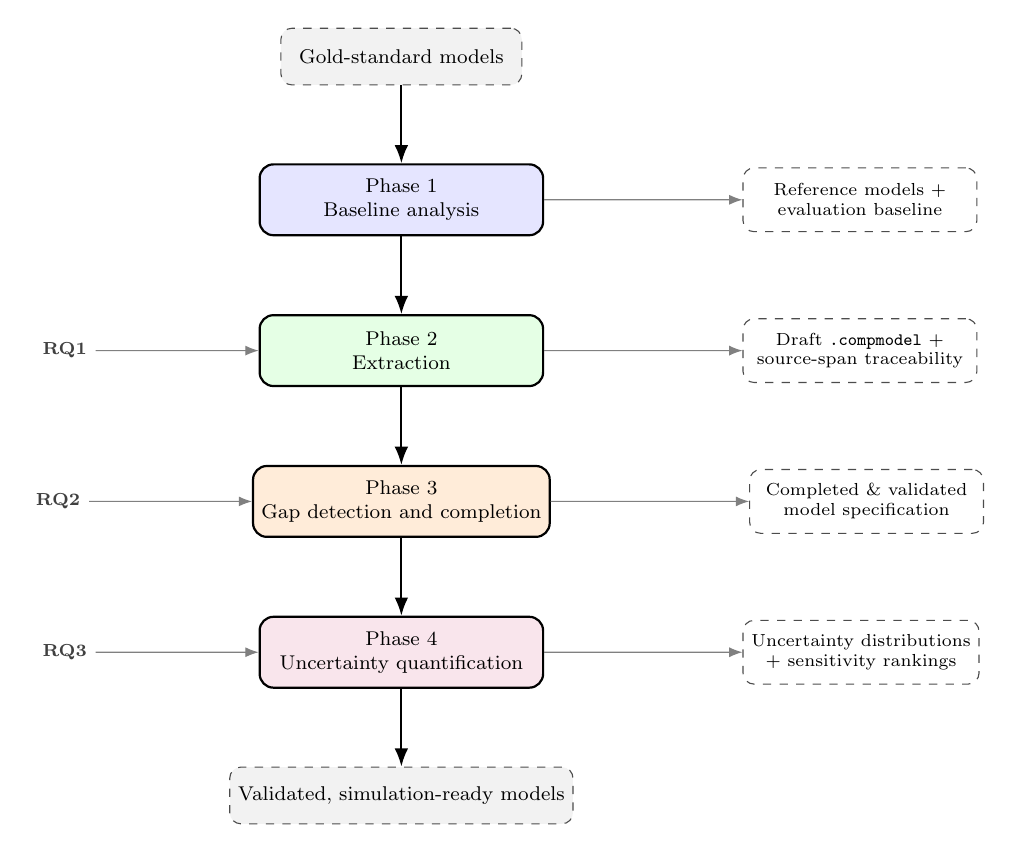
\begin{tikzpicture}[
    scale=0.9,
    transform shape,
    node distance=1.1cm,
    >={Latex},
    box/.style={
        rectangle,
        rounded corners=5pt,
        draw=black,
        thick,
        minimum width=4.0cm,
        minimum height=1.0cm,
        align=center,
        font=\footnotesize
    },
    resultbox/.style={
        rectangle,
        rounded corners=4pt,
        draw=black!70,
        dashed,
        minimum width=3.3cm,
        minimum height=0.9cm,
        align=center,
        font=\scriptsize
    },
    io/.style={
        rectangle,
        rounded corners=4pt,
        draw=black!70,
        dashed,
        minimum width=3.4cm,
        minimum height=0.8cm,
        align=center,
        font=\footnotesize
    },
    rq/.style={
        font=\scriptsize\bfseries,
        text=black!75
    }
]

% Main vertical pipeline
\node[io, fill=gray!10] (input) {Gold-standard models};

\node[box, fill=blue!10, below=of input] (p1) {Phase 1\\Baseline analysis};

\node[box, fill=green!10, below=of p1] (p2) {Phase 2\\Extraction};

\node[box, fill=orange!15, below=of p2] (p3) {Phase 3\\Gap detection and completion};

\node[box, fill=purple!10, below=of p3] (p4) {Phase 4\\Uncertainty quantification};

\node[io, fill=gray!10, below=of p4] (output) {Validated, simulation-ready models};

% Main arrows
\draw[->, thick] (input) -- (p1);
\draw[->, thick] (p1) -- (p2);
\draw[->, thick] (p2) -- (p3);
\draw[->, thick] (p3) -- (p4);
\draw[->, thick] (p4) -- (output);

% Left side: RQs as plain labels
\node[rq, left=2.3cm of p2] (rq1) {RQ1};
\node[rq, left=2.3cm of p3] (rq2) {RQ2};
\node[rq, left=2.3cm of p4] (rq3) {RQ3};

\draw[->, thin, gray] (rq1.east) -- (p2.west);
\draw[->, thin, gray] (rq2.east) -- (p3.west);
\draw[->, thin, gray] (rq3.east) -- (p4.west);

% Right side: result boxes
\node[resultbox, right=2.8cm of p1] (r1) {Reference models +\\evaluation baseline};
\node[resultbox, right=2.8cm of p2] (r2) {Draft \texttt{.compmodel} +\\source-span traceability};
\node[resultbox, right=2.8cm of p3] (r3) {Completed \& validated\\model specification};
\node[resultbox, right=2.8cm of p4] (r4) {Uncertainty distributions\\+ sensitivity rankings};

\draw[->, thin, gray] (p1.east) -- (r1.west);
\draw[->, thin, gray] (p2.east) -- (r2.west);
\draw[->, thin, gray] (p3.east) -- (r3.west);
\draw[->, thin, gray] (p4.east) -- (r4.west);

\end{tikzpicture}
\caption{High-level overview of the proposed pipeline. Each phase is associated with its corresponding research question on the left and its main output on the right.}
\label{fig:pipeline_overview}
\end{figure}

\subsection{Evaluation plan}

I will compare pipeline outputs to \textbf{reference models} that a human authored for each benchmark paper. Those models will be the ground truth for compartments, flows, and parameters in all quantitative scoring and in identifying missing structure.

The plan addresses three levels. First, I will ask whether assisted extraction recovers the right structure compared to the reference (Phase 2, RQ1). Second, I will ask whether completion narrows gaps and improves numeric agreement (Phase 3, RQ2). Third, for models that simulate correctly, I will examine what uncertainty and sensitivity analyses show about epidemic outputs (Phase 4, RQ3). I will compute metrics \textbf{per paper}, then summarize by disease and for the full benchmark corpus.

\textbf{Link to users of the method.} High structural recall and sound wiring are not abstract scores: they indicate whether a practitioner could \textbf{reuse} a draft model with limited repair, whether repeated runs yield \textbf{reproducible} structure under fixed configuration, and whether automation reduces manual transcription effort (\textbf{productivity}). I will interpret completeness and gap categories in these terms where the evidence supports it, and I will tie each experimental block to what it shows about tool-supported modeling from documents rather than only to internal benchmarks.

\paragraph{Phase 2 (RQ1).}
I will measure structural agreement with recall, precision, and F1 over compartment names and over flows between compartments. I will align names with \textbf{fuzzy matching} and light normalization so minor wording differences (for example ``I'' versus ``Infected'') do not dominate the score \citep{python_difflib}. I will run the same paper with different LLM providers where appropriate to study robustness. When a run stores the paper passages linked to each extracted entity, I will use error analysis on those passages to explain individual mistakes (ambiguous wording, noisy text, unsupported inference), not only report aggregate scores.

\paragraph{Phase 3 (RQ2).}
I will compare the draft model and extracted entities to the reference before filling: I will list missing compartments, flows, parameters, or wiring. After filling, I will recompute structural scores to assess whether completion improved the draft. I will classify numeric values suggested for parameters against the reference (for example exact, close, approximate, or poor). I will optionally contrast retrieval-driven filling, LLM-only filling, and combined strategies to see which parts of the method matter. I will include a short qualitative section that groups remaining failures (for example flows not connected in the equations, inconsistent units) alongside the numeric tables.

\paragraph{Phase 4 (RQ3).}
For models that integrate and run without numerical failure, I will use Monte Carlo simulation to obtain distributions over summary quantities of interest (for example epidemic peak time, peak prevalence, cumulative incidence). I will perform \textbf{sensitivity analysis} using one-at-a-time screening of rates \citep{morris1991factorial} to rank which parameters most influence those outputs. I will flag separately runs that produce flat trajectories, non-finite values, or obvious inconsistency between parameters and dynamics so they are not mistaken for meaningful uncertainty.

\paragraph{Reproducibility (RQ4).}
I will record LLM provider, model family, and key generation settings, together with software versions or revision identifiers for the pipeline. I will state choices about PDF text extraction (for example use of structured parsing tools \citep{romary2015grobid}) so others can interpret extraction noise.

\paragraph{What will count as success.}
Success is not only higher scores on a benchmark, but whether the method produces models that are actually useful in practice. The evaluation therefore focuses on whether the pipeline can generate models that are complete enough to reuse, reduce manual effort, and can be reproduced under the same setup.

The main quantity I will measure is \textbf{structural completeness}, using recall and precision on compartments and flows, together with numeric agreement on parameters relative to reference models. These results are then interpreted in terms of how a user would work with the output.

\textbf{Reusability} is supported when a draft model is mostly complete and correctly wired, so that a practitioner can use it with only minor fixes. In this case, most of the model has effectively been recovered from the paper.

\textbf{Productivity} is supported when completion reduces the amount of missing structure and parameter specification that would otherwise need to be added manually. Improvements from extraction to completion indicate that the pipeline saves time compared to building the model from scratch.

\textbf{Reproducibility} is supported when repeated runs with the same configuration produce similar structures and scores, and when all settings and outputs are recorded so that results can be reproduced by others.

Uncertainty and sensitivity analysis are only treated as meaningful when they are applied to models that pass basic validation checks. This ensures that the resulting plots describe the behavior of a consistent model rather than artifacts of extraction or completion errors. Throughout, simulation results are used to illustrate the behavior of the pipeline and not to support clinical or policy conclusions \citep{Ferguson2006Influenza}.


% ---------------------------------------------------------------------------
\section{Expected contributions}
% ---------------------------------------------------------------------------

\begin{itemize}[leftmargin=*]
  \item \textbf{Integrated pipeline.} I will deliver a documented end-to-end workflow from baseline analysis through extraction, completion, validation, and uncertainty quantification for compartmental epidemiological models.
  \item \textbf{Benchmarks and evaluation.} I will report empirical results across multiple diseases and papers, with clear metrics and discussion of disease-specific difficulty and failure modes.
  \item \textbf{Methodological clarity.} I will give explicit treatment of validation choices and simulation pitfalls (e.g.\ degenerate parameters, initial conditions, and parameter flow connectivity).
  \item \textbf{Reproducibility.} I will provide open-source-style documentation (e.g.\ READMEs, fixed pipelines) that support replication and extension by others.
\end{itemize}

The primary beneficiaries are \textbf{modelers}, \textbf{computational epidemiology researchers}, and \textbf{educators} who work with compartmental models. The proposed method will improve the process of turning published studies into executable models by reducing the amount of manual transcription and interpretation required.

For practitioners, the pipeline will support \textbf{faster model construction} by recovering a large portion of the model structure directly from the source document, allowing effort to shift from transcription to validation and analysis. It will also improve \textbf{traceability}, since each model element can be linked back to specific passages in the paper, making assumptions easier to check and justify.

For researchers, the method will support \textbf{reproducibility and comparability} by producing structured models under fixed configurations, together with recorded settings and evaluation results. This will make it easier to compare modeling assumptions across papers and to replicate results without rebuilding models from scratch.

For teaching and learning, the pipeline will provide a clearer connection between published descriptions and formal models, which can help students understand how compartmental systems are constructed and validated in practice.

Overall, the work will improve the workflow from document-level requirements to analysis-ready models by making it more systematic, less error-prone, and easier to reproduce, while still leaving final modeling decisions to domain experts.

% ---------------------------------------------------------------------------
\section{Timeline}
% ---------------------------------------------------------------------------

I will follow a plan spanning \textbf{24 months}. I will reserve the
\textbf{last two months (Months 23 and 24)} for committee review, final
revisions, formatting, and thesis submission; I will not schedule new
experiments or major new analysis in that period. I will shift month labels
to match my official start date.

The work is organized into four main phases:

\textbf{Phase 1 (Months 1--5):} Literature consolidation, scope definition,
evaluation protocol design, and reproduction of Phases 1 and 2 baseline experiments.

\textbf{Phase 2 (Months 6--10):} Extraction studies across providers and benchmark
papers, metric computation, error analysis, and drafting of extraction and
evaluation methods.

\textbf{Phase 3 (Months 11--15):} Construction of the paper database and
rule-based retrieval system, LLM-based gap filling, validation against gold
standards, and ablation and failure-mode analysis.

\textbf{Phase 4 (Months 16--20):} Uncertainty quantification, sensitivity
analysis, benchmark integration, and drafting of results chapters and figures.

\textbf{Finalization (Months 21--24):} Thesis integration, incorporation of
supervisor feedback, polishing, committee review, final revisions, formatting,
and submission.

Figure~\ref{fig:timeline} summarizes the schedule.

\begin{figure}[H]
\centering
\resizebox{0.85\textwidth}{!}{
\begin{ganttchart}[
    x unit=0.5cm,
    y unit title=0.6cm,
    y unit chart=0.8cm,
    vgrid,
    hgrid,
    title height=0.8,
    bar height=0.6,
    bar label font=\small\bfseries,
    title label font=\small
]{1}{24}

\gantttitle{Twenty-four-month plan}{24} \\
\gantttitlelist{1,...,24}{1} \\

% Color definitions
\definecolor{phaseone}{RGB}{66,135,245}
\definecolor{phasetwo}{RGB}{52,168,83}
\definecolor{phasethree}{RGB}{251,188,5}
\definecolor{phasefour}{RGB}{234,67,53}
\definecolor{finalphase}{RGB}{120,120,120}

% Bars
\ganttbar[bar/.append style={fill=phaseone}]{Phase 1}{1}{5} \\
\ganttbar[bar/.append style={fill=phasetwo}]{Phase 2}{6}{10} \\
\ganttbar[bar/.append style={fill=phasethree}]{Phase 3}{11}{15} \\
\ganttbar[bar/.append style={fill=phasefour}]{Phase 4}{16}{20} \\
\ganttbar[bar/.append style={fill=finalphase}]{Finalization}{21}{24}

\end{ganttchart}
}
\caption{Twenty-four-month plan.}
\label{fig:timeline}
\end{figure}

\bibliographystyle{plainnat}
\bibliography{refs}

\end{document}
